\gls{wrtc} deviates from traditional enterprise collaboration systems by opening up communications from web applications instead of controlled software pieces. So how do we make the open web interoperate with the closed enterprise world. There are two ways of going about this problem. We can either choose to redo the whole existing architecture of the enterprise collaboration system putting \gls{wrtc} technology in the center and upgrade all the existing infrastructure to support \gls{wrtc}, but this is an expensive solution, especially since the \gls{ietf} has not yet finished deciding upon which protocols and codecs to be used. Therefore, the best option is to extend current architecture with \gls{wrtc} capabilities. To do this we have to create a gateway between the underlying technologies of \gls{wrtc} specified as \gls{rtcweb} and existing enterprise infrastructure. The aim when creating a gateway between the two systems is to re-use as much as possible of existing architecture. This chapter acts as an intro to this problem.

\section{Research problems}
There are basically three translating components we have to create: the signaling proxy, the transport proxy, and the transcoder. We also have to figure out how to cross the enterprise firewall. Once we have achieved that, we can also look into how to develop a WebRTC client for mobile devices. The signaling proxy is the offer/answer exchange of messages. The transport proxy will handle the transportation of media and gathering of ICE candidates, and the transcoder will simply transcode media between different formats. In Figure \ref{fig:gateway-layers} we can see where the interworking components has to go (marked with a ?) in such an architecture. We will place the gateway behind the enterprise firewall to have more control of the media. If we start by looking at how to receive WebRTC traffic, we first we have to figure out how to cross the enterprise firewall, then translation, and lastly we can look at developing a client for mobile devices. I've chosen not to include images of the STUN and TURN servers as these are parts of the ICE technique.
\\
\begin{figure}[here]
\centerline{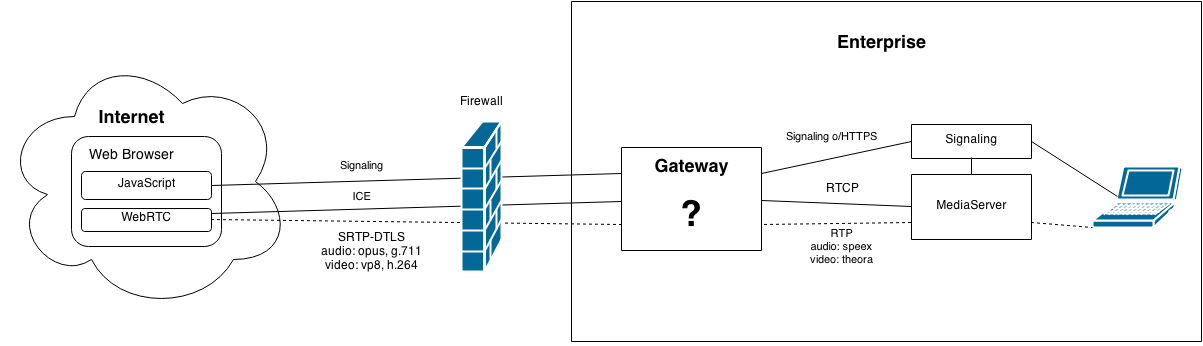
\includegraphics[scale=0.39]{gateway-unknown.png}}
\caption{WebRTC-Enterprise gateway placement}
\label{fig:gateway-layers}
\end{figure}

\subsection{The Enterprise Firewall}
We have to handle incoming signaling, this should not be a problem since the traffic runs over HTTP. We also have to handle incoming ICE requests from a STUN server. In VA the firewall on the client side is manually configured to have open connections on specific ports. This approach would not be applicable for mobile devices that change their IP address all the time, depending on which network they are currently connected to. WebRTC solves this by utilizing a STUN server that gathers ICE candidates to bypass the NAT/firewall for transportation of media. In the enterprise world a \gls{sbc} is commonly used to control incoming media traffic. WebRTC media flows would probably be blocked by most \gls{sbc}s, so we have to find some way of detecting and applying policy to WebRTC media flows. This is a bigger topic that I will go more deeply into in the next chapter.

\subsection{The Signaling Proxy}
First we have to figure out how to authenticate the users. VA uses Kerberos authentication, so we need to figure out how to do this in the browser. Secondly we need to translate the signaling. \gls{wrtc} does not define any standard way of doing signaling, but we do have to implement it and get it working with typical enterprise ways of doing this. One of the best low latency ways of doing messaging in the browser today is by using WebSockets over HTTP. This then needs to be translated to VA's way of doing signaling. Lastly we need to handle negotiating the SDP. The SDP should be included in the messages exchanged through signaling.
 

\subsection{The Transport Proxy}
In the \gls{wrtc} world the media plane is designed to avoid having to relay media streams. The goal is to have pure peer-to-peer connections, while in the enterprise world it is common to have full control over the media plane and in most cases use some kind of media server. Also the \gls{wrtc} specification says that support for \gls{ice} and \gls{srtp}-\gls{dtls} are mandatory. Encryption is hardly ever used in the enterprise world, so this is another challenge. If encryption is used, it is more common to use \gls{srtp}-\gls{sdes} with the keys being handled on the signaling plane, rather than in the media plane that is the case with \gls{dtls}. We also need to both decrypt and encrypt the media streams from SRTP to RTP and vice versa. \gls{wrtc} uses one-way media streams, while an enterprise system usually expects to receive bi-directional streams. This can be fixed by multiplexing the streams, so we can have multiple streams running over the same network port.

\subsection{The Transcoder}
The biggest issues here is probably which codecs we need to implement. The \gls{ietf} has landed on two default audio codecs, but has not as of 16th of May decided on which video codec to use yet. The most typical enterprise video codec used is H.264. Right now the \gls{ietf} are deciding between VP8 and H.264, so currently we have to support both and do transcoding between them. In VA's case we need to implement the Speex and Theora codecs as well.

In Figure \ref{fig:gateway} we see the suggested gateway components.
\\
\begin{figure}[here]
\centerline{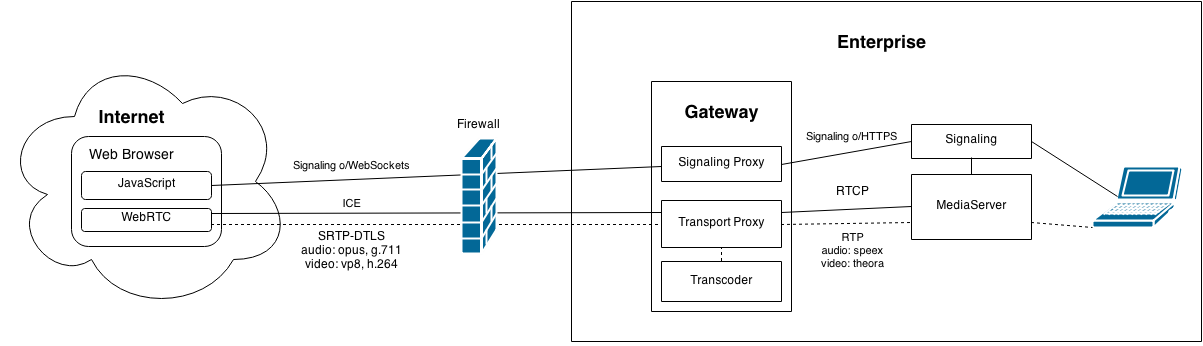
\includegraphics[scale=0.4]{gateway-suggested.png}}
\caption{WebRTC-Enterprise gateway}
\label{fig:gateway}
\end{figure}

\section{Summary}
The first iteration of \gls{rtcweb} is still under development, and not all protocols and codecs have been decided yet. It is theoretically possible to create a gateway and it has been done before, but mostly under closed source. Some of the biggest issues are how to handle the signaling, translation of the media, and crossing the enterprise firewall. In the next chapters I will dive further into each component mentioned above.
